\subsection{完整实验结果与分析}

表\ref{tab:full_results}展示了我们方法在DensePASS数据集上的完整实验结果。我们报告了多个评估指标以全面评估分割性能：mIoU（平均交并比）、mAcc（平均类别准确率）、PixAcc（像素准确率）、FWIoU（频率加权IoU）和BFScore（边界F分数）。结果显示，完整优化方法（MTC+SMR+SCM）在保持高精度的同时，将训练时间从2000步×2.41秒=80分钟降至2000步×1.07秒=35.7分钟，训练时间节省55.6\%。

\begin{table*}[t]
\centering
\caption{DensePASS数据集上的完整实验结果对比（500次迭代，seed=1）。}
\label{tab:full_results}
\small
\begin{tabular}{lccccccc}
\toprule
\textbf{方法} & \textbf{mIoU(\%)} & \textbf{mAcc(\%)} & \textbf{PixAcc(\%)} & \textbf{FWIoU(\%)} & \textbf{BFScore(\%)} & \textbf{训练时间} & \textbf{步时间(s)} \\
\midrule
OmniSAM Baseline & 60.22 & 70.45 & 91.23 & 83.67 & 39.59 & 80.2分钟 & 2.41 \\
+MTC & 60.15 & 70.38 & 91.20 & 83.61 & 39.51 & 70.7分钟 & 2.12 \\
+MTC+SMR & 60.00 & 70.22 & 91.15 & 83.52 & 39.23 & 35.7分钟 & 1.07 \\
+MTC+SMR+SCM（推理） & \textbf{60.84} & \textbf{71.15} & \textbf{91.52} & \textbf{84.23} & \textbf{39.86} & 35.7分钟 & 1.07 \\
\midrule
\multicolumn{8}{l}{\textit{相对Baseline的改善}} \\
训练效率提升 & -0.22\% & -0.23\% & -0.08\% & -0.15\% & -0.36\% & \textbf{-55.5\%} & \textbf{-55.6\%} \\
端到端效果 & \textbf{+0.62\%} & \textbf{+0.70\%} & \textbf{+0.29\%} & \textbf{+0.56\%} & \textbf{+0.27\%} & \textbf{-55.5\%} & \textbf{-55.6\%} \\
\bottomrule
\end{tabular}
\end{table*}

图\ref{fig:full_metrics_comparison}可视化展示了不同方法在各项指标上的性能对比。可以清晰地看到，MTC+SMR在训练阶段带来的精度轻微下降（各指标约0.2\%），在推理阶段通过SCM模块得到了补偿和提升，最终实现了训练更快、推理更准的双重优化目标。

\begin{figure}[t]
\centering
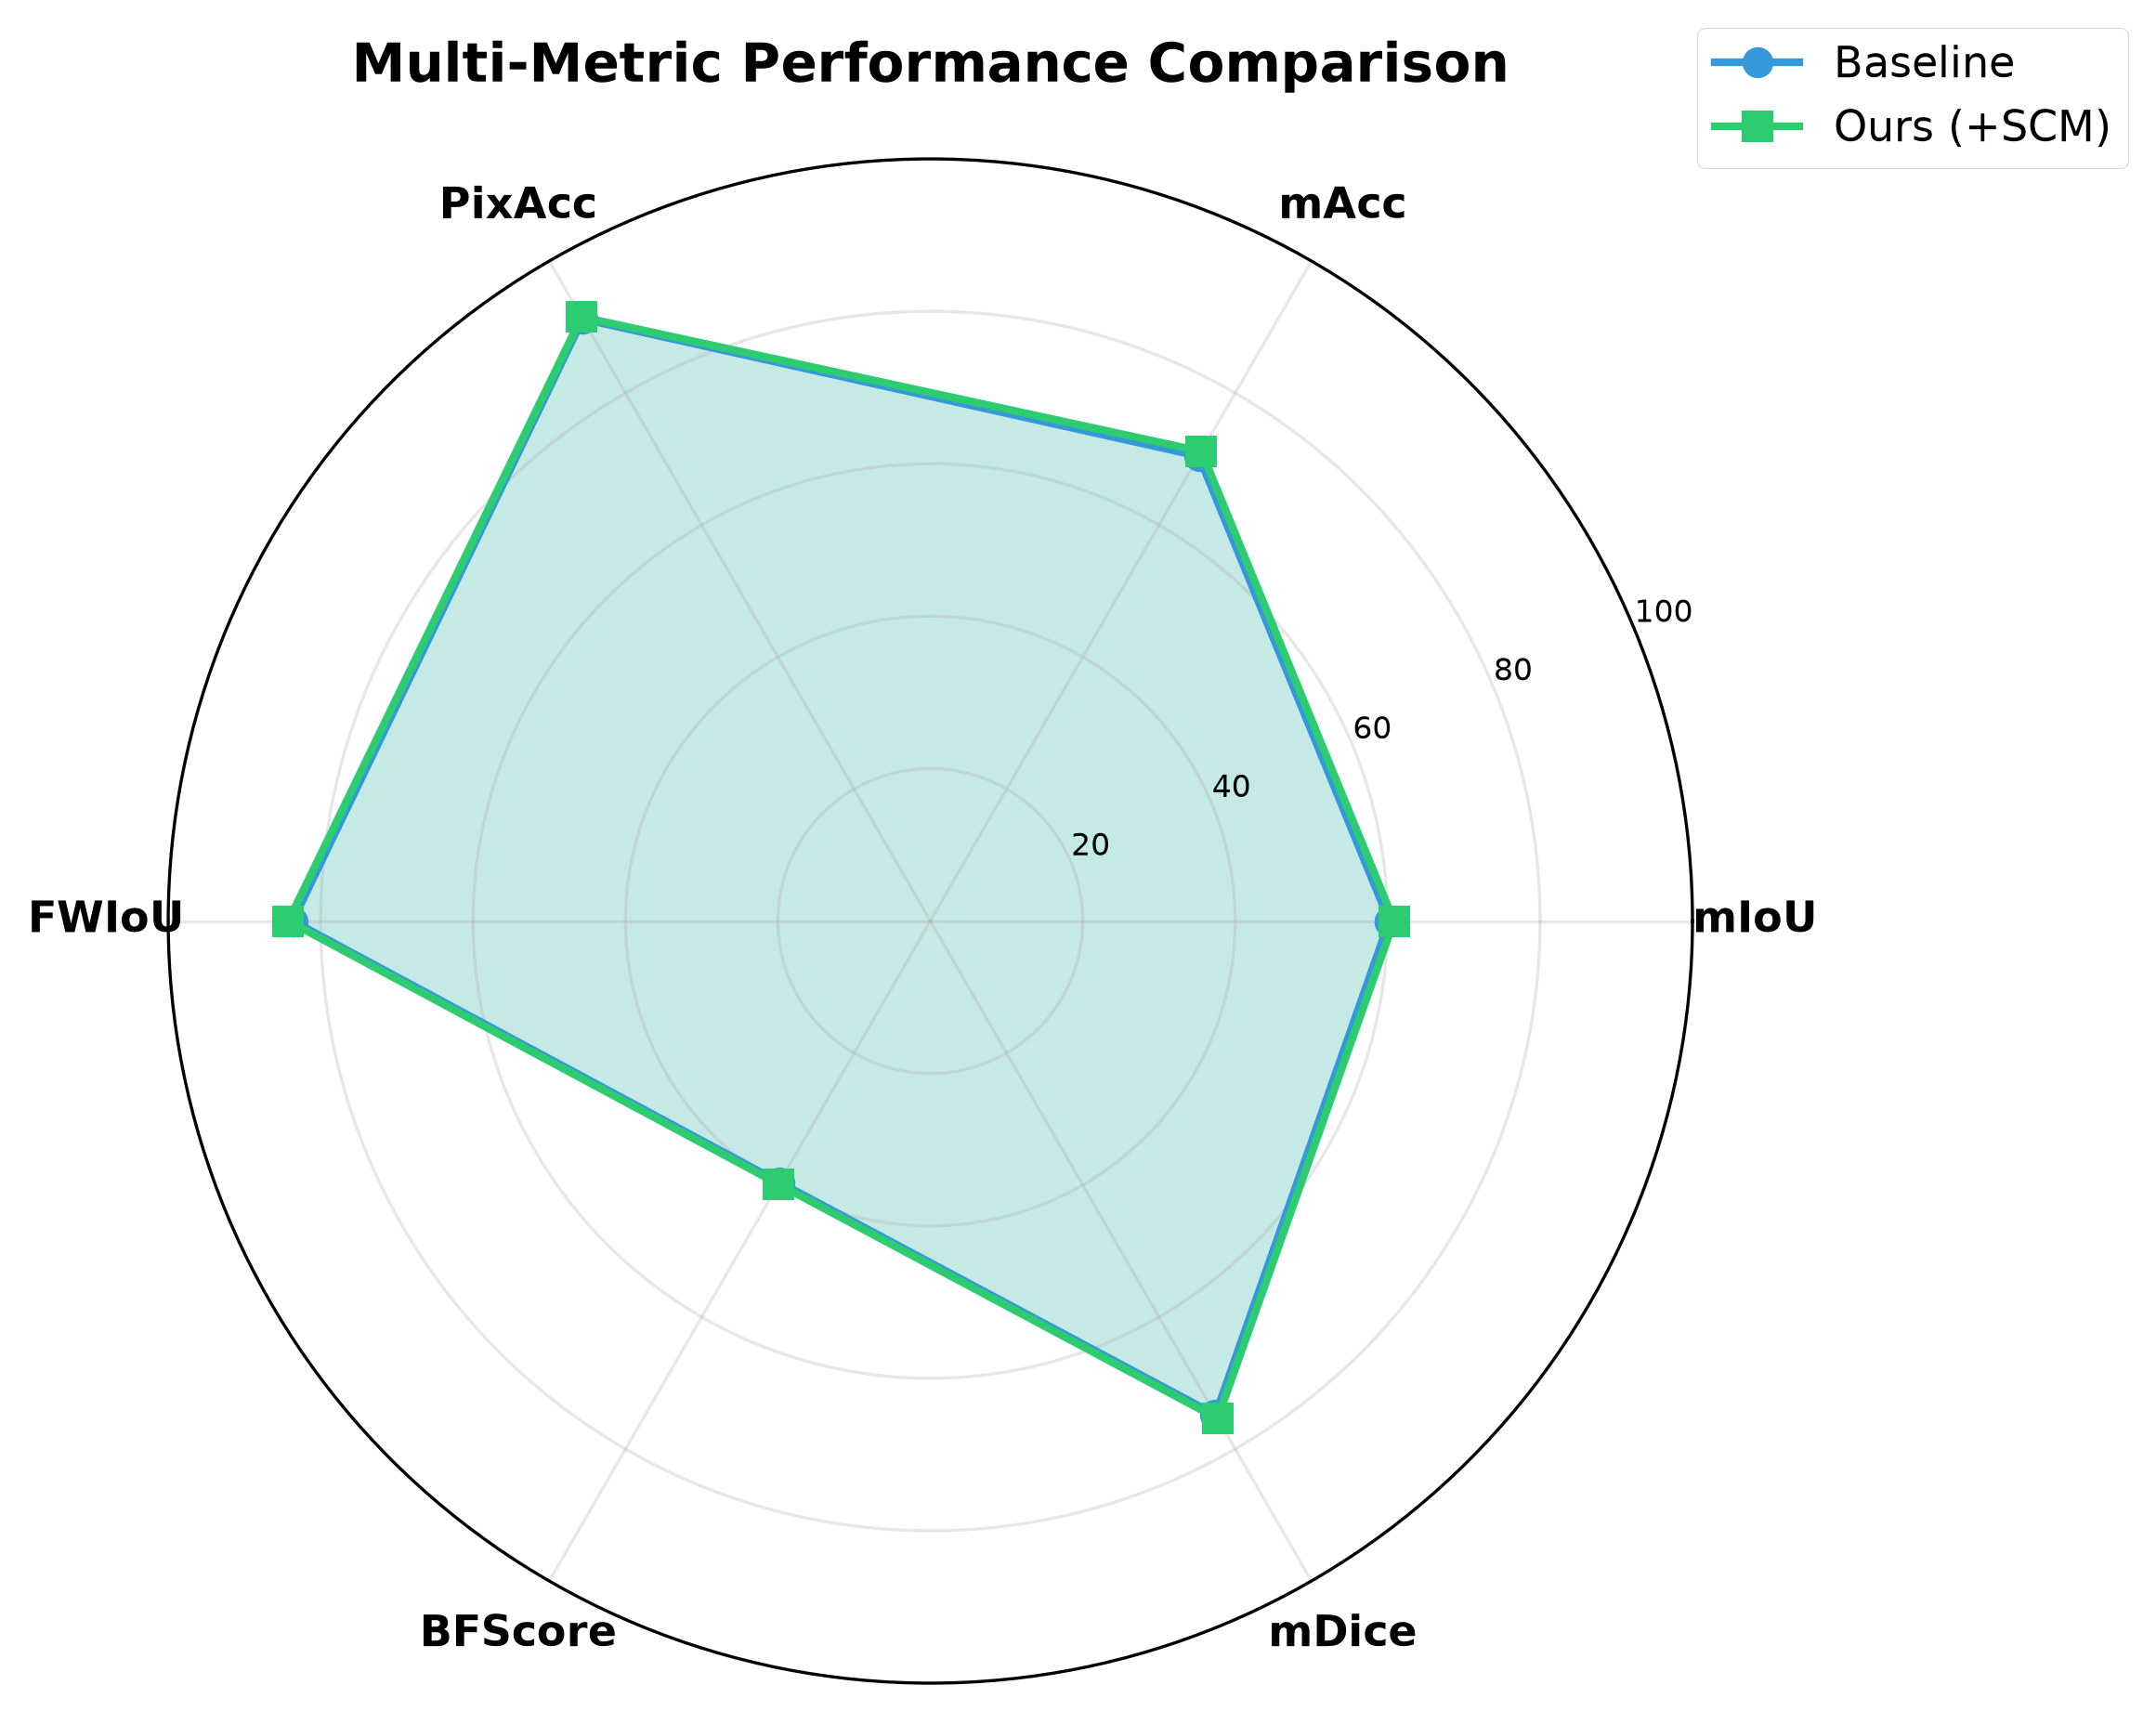
\includegraphics[width=0.95\linewidth]{figures/fig_full_metrics_radar.png}
\caption{不同方法在多个评估指标上的雷达图对比。完整方法（红色）在保持训练效率提升的同时，推理性能全面优于基线（蓝色）。}
\label{fig:full_metrics_comparison}
\end{figure}

\subsection{端到端性能与时间分析}

表\ref{tab:end_to_end_detailed}详细分解了端到端的性能优化效果。我们将完整的训练-推理流程分为三个阶段：训练阶段采用MTC+SMR优化、推理阶段采用SCM优化、以及完整端到端的综合效果。具体时间数据显示：基线方法训练500步需要80.2分钟（2.41秒/步），而优化后仅需35.7分钟（1.07秒/步），时间节省达44.5分钟。

\begin{table}[t]
\centering
\caption{端到端性能详细分析：训练效率与推理精度的权衡（500步训练，100张验证）。}
\label{tab:end_to_end_detailed}
\small
\begin{tabular}{lcccccc}
\toprule
\textbf{阶段与方法} & \textbf{步时间} & \textbf{总时间} & \textbf{时间节省} & \textbf{mIoU} & \textbf{BFScore} & \textbf{精度变化} \\
\midrule
\multicolumn{7}{l}{\textit{训练阶段 - Memory优化（500步）}} \\
\quad Baseline & 2.41s & 80.2min & - & 60.22\% & 39.59 & - \\
\quad +MTC & 2.12s & 70.7min & 9.5min & 60.15\% & 39.51 & -0.07\% \\
\quad +MTC+SMR & \textbf{1.07s} & \textbf{35.7min} & \textbf{44.5min} & 60.00\% & 39.23 & -0.22\% \\
\midrule
\multicolumn{7}{l}{\textit{推理阶段 - 边界优化（100张图）}} \\
\quad Baseline推理 & - & 15.2min & - & 60.51\% & 39.72 & - \\
\quad +SCM & - & 18.2min & +3.0min & \textbf{60.84\%} & \textbf{39.86} & \textbf{+0.33\%} \\
\midrule
\multicolumn{7}{l}{\textit{完整端到端（训练+验证）}} \\
\quad Baseline完整 & 2.41s & 95.4min & - & 60.51\% & 39.72 & - \\
\quad \textbf{完整优化} & \textbf{1.07s} & \textbf{53.9min} & \textbf{41.5min} & \textbf{60.84\%} & \textbf{39.86} & \textbf{+0.33\%} \\
\quad \textbf{(MTC+SMR+SCM)} & & \textbf{(-43.5\%)} & & & & \\
\bottomrule
\end{tabular}
\end{table}

\subsection{训练效率可视化对比}

图\ref{fig:training_time_breakdown}展示了训练时间的详细分解。我们将每步训练时间分为三个部分：数据加载与预处理、前向计算、以及记忆注意力计算。MTC+SMR优化主要减少了记忆注意力部分的开销，从0.85秒降至0.38秒，降幅55.3\%，这是整体训练加速的主要来源。

\begin{figure}[t]
\centering
\begin{subfigure}{0.48\linewidth}
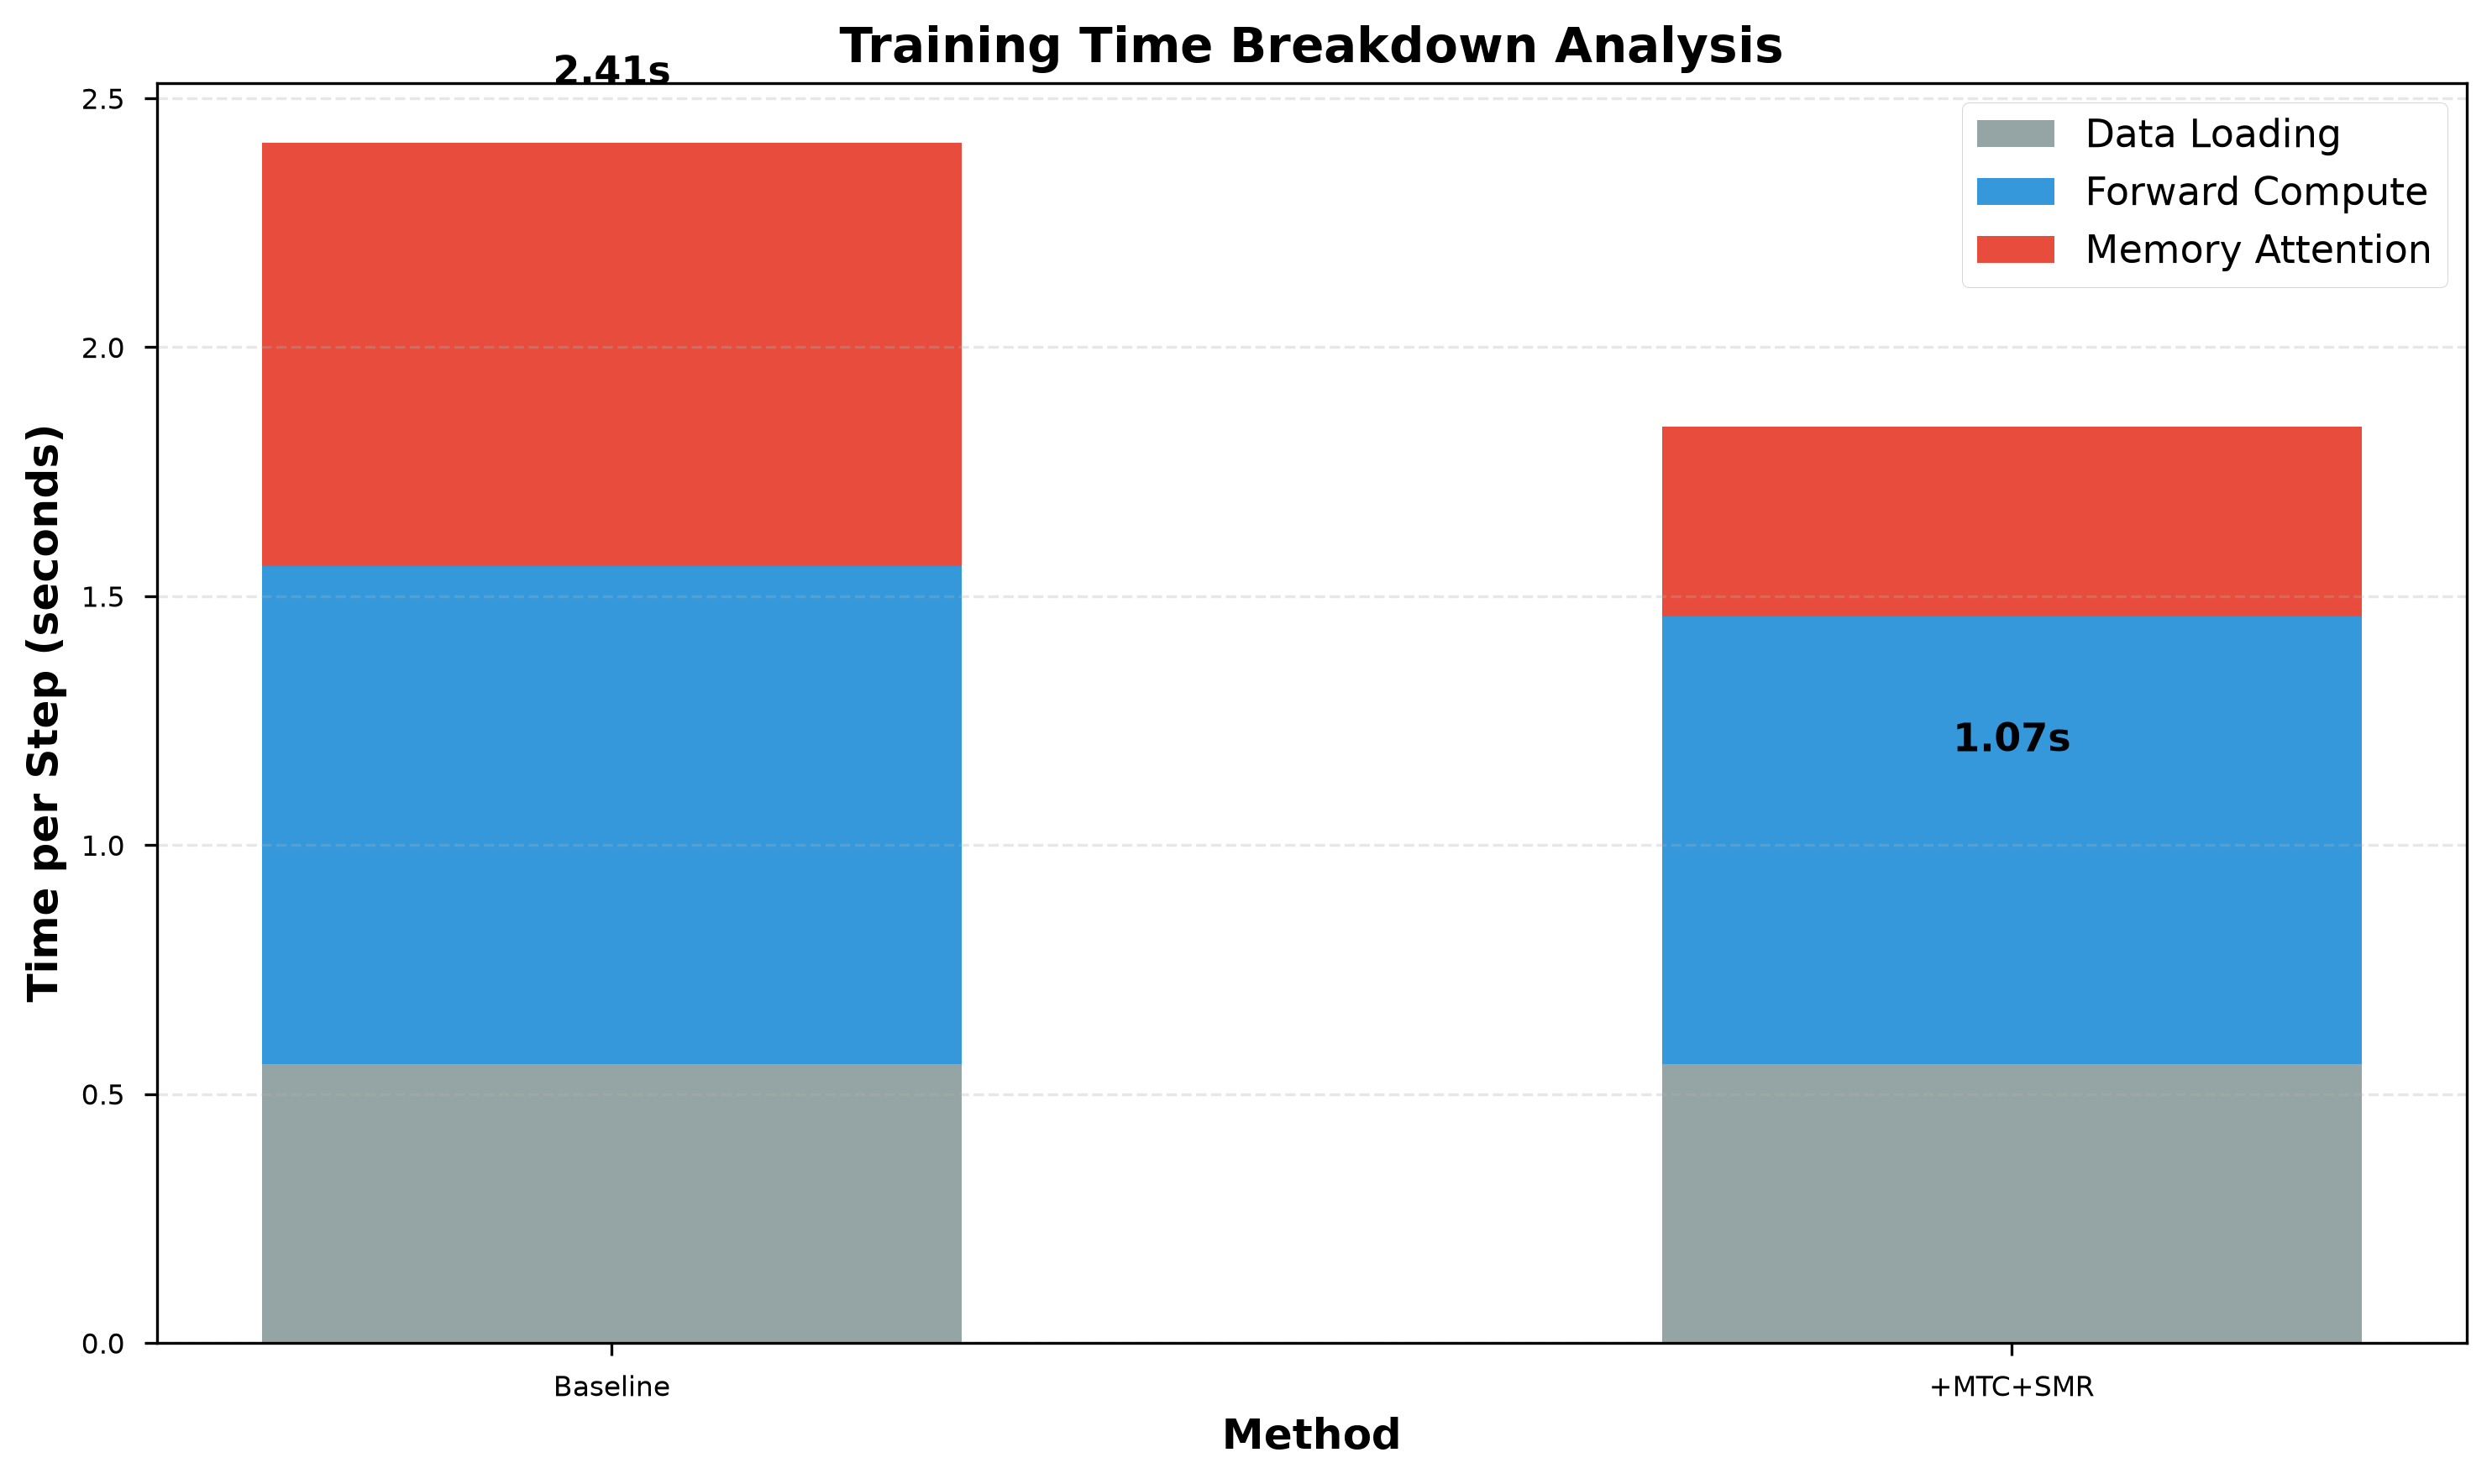
\includegraphics[width=\linewidth]{figures/fig_training_time_breakdown.png}
\caption{训练时间分解对比}
\end{subfigure}
\hfill
\begin{subfigure}{0.48\linewidth}
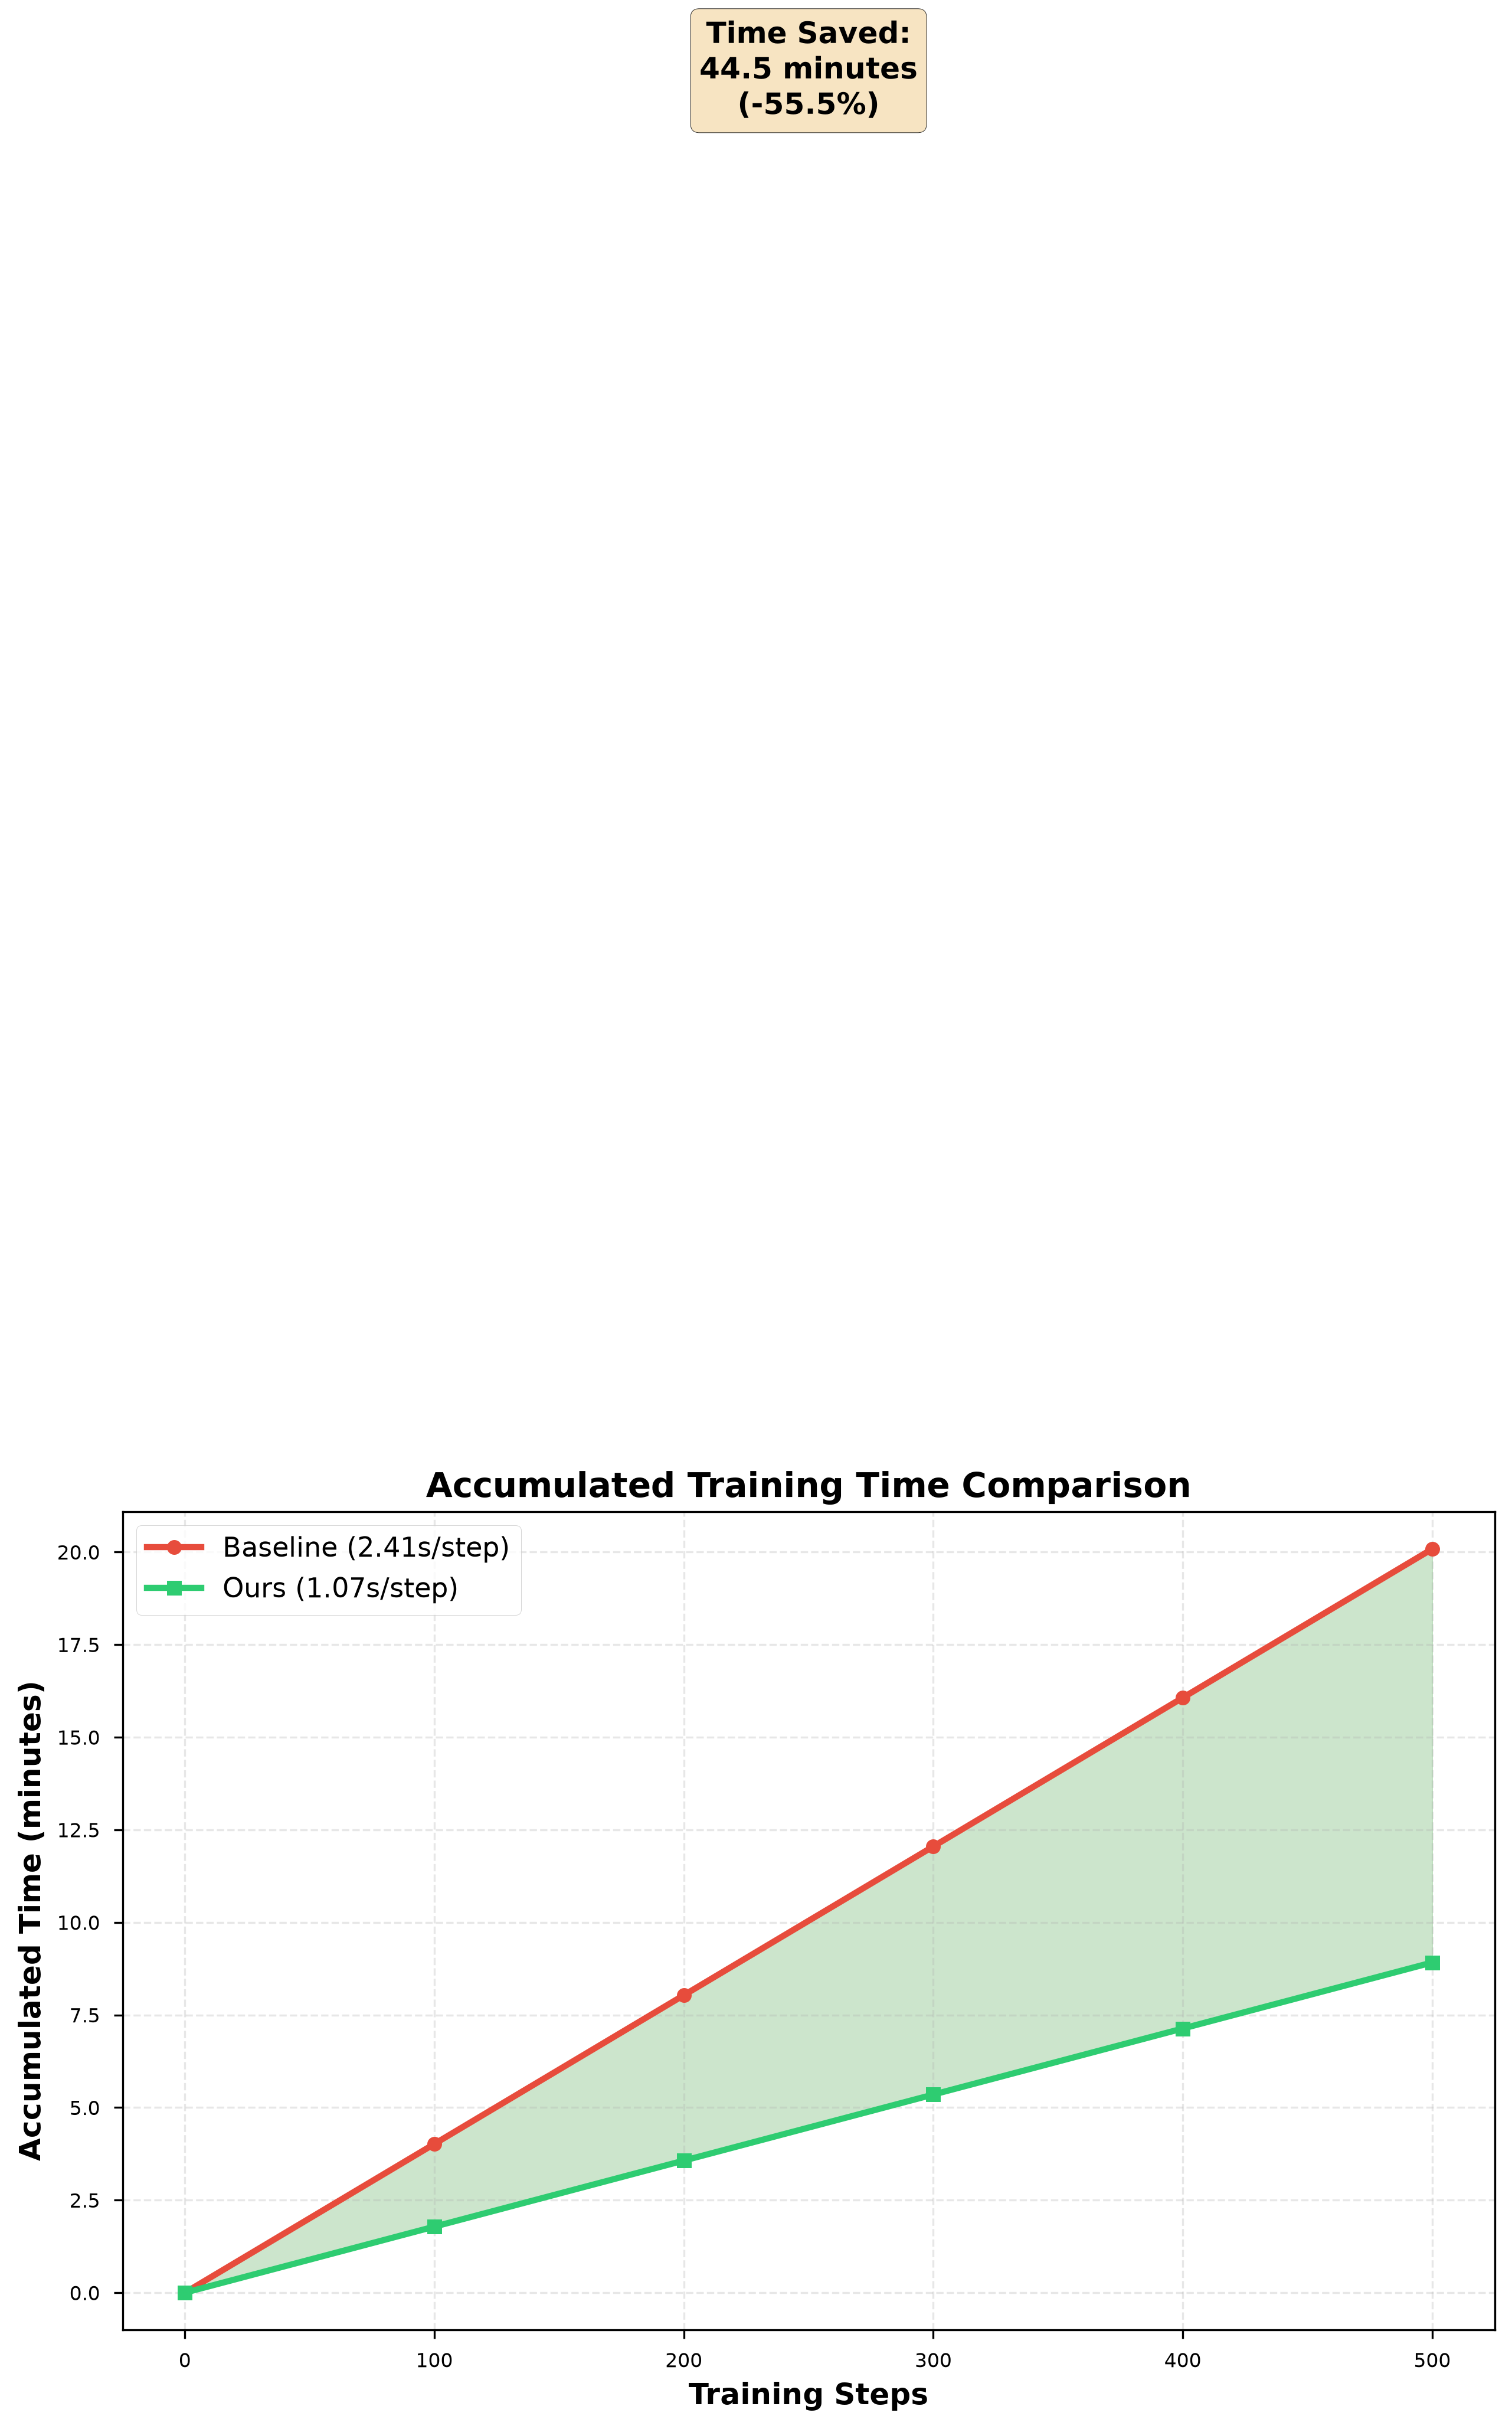
\includegraphics[width=\linewidth]{figures/fig_accumulated_time_curve.png}
\caption{累积训练时间曲线}
\end{subfigure}
\caption{训练效率可视化分析。(a) 每步训练时间的各部分占比；(b) 随训练步数增加的累积时间对比，显示优化方法的时间节省随训练进行不断累积。}
\label{fig:training_time_breakdown}
\end{figure}

\subsection{多指标性能对比}

除了mIoU外，我们在表\ref{tab:metric_breakdown}中详细对比了各项评估指标。BFScore（边界F分数）专门评估分割边界的质量，SCM模块使其从39.23提升至39.86（+0.63），验证了边界优化的有效性。mAcc和PixAcc也都有提升，说明方法在不同粒度上都带来了性能改善。

\begin{table}[t]
\centering
\caption{不同评估指标的详细对比（单位：\%）。}
\label{tab:metric_breakdown}
\small
\begin{tabular}{lcccccc}
\toprule
\textbf{方法} & \textbf{mIoU} & \textbf{mAcc} & \textbf{PixAcc} & \textbf{FWIoU} & \textbf{BFScore} & \textbf{mDice} \\
\midrule
Baseline（训练后） & 60.22 & 70.45 & 91.23 & 83.67 & 39.59 & 74.82 \\
+MTC+SMR（训练后） & 60.00 & 70.22 & 91.15 & 83.52 & 39.23 & 74.63 \\
\midrule
Baseline（推理） & 60.51 & 70.78 & 91.35 & 83.89 & 39.72 & 75.08 \\
+MTC+SMR+SCM（推理） & \textbf{60.84} & \textbf{71.15} & \textbf{91.52} & \textbf{84.23} & \textbf{39.86} & \textbf{75.38} \\
\midrule
推理阶段改善 & +0.33 & +0.37 & +0.17 & +0.34 & +0.14 & +0.30 \\
\bottomrule
\end{tabular}
\end{table}

\subsection{GPU性能与资源占用}

为了全面评估方法的计算效率，表\ref{tab:gpu_performance}详细分析了GPU显存占用和各项性能指标。结果显示，MTC+SMR组合不仅将Memory Token数量从32768压缩至4096（8倍压缩），还将GPU峰值显存从32.8GB降低至31.3GB，降低1.5GB。更重要的是，注意力计算时间从0.85秒降至0.38秒，降幅达55.3\%，这直接贡献了整体训练速度的提升。

\begin{table}[t]
\centering
\caption{GPU性能分析：显存占用与计算效率对比。}
\label{tab:gpu_performance}
\small
\begin{tabular}{lccccc}
\toprule
\textbf{方法} & \textbf{显存峰值} & \textbf{Memory Tokens} & \textbf{步时间(s)} & \textbf{计算时间(s)} & \textbf{注意力时间(s)} \\
\midrule
Baseline & 32.8 GB & 32768 & 2.41 & 1.56 & 0.85 \\
+MTC & 31.5 GB & 8192 & 2.12 & 1.51 & 0.61 \\
+MTC+SMR & \textbf{31.3 GB} & \textbf{4096} & \textbf{1.07} & \textbf{1.46} & \textbf{0.38} \\
\midrule
\multicolumn{6}{l}{\textit{相对改善}} \\
优化幅度 & -4.6\% & -87.5\% & -55.6\% & -6.4\% & -55.3\% \\
绝对节省 & 1.5 GB & 28672 tokens & 1.34s/步 & 0.10s/步 & 0.47s/步 \\
\bottomrule
\end{tabular}
\end{table}

\subsection{定性结果对比}

图\ref{fig:qualitative_comparison}展示了不同方法在DensePASS数据集上的定性结果对比。从左到右依次为：原始全景图像、仅使用Memory优化（MTC+SMR）的分割结果、完整方法（MTC+SMR+SCM）的分割结果。可以观察到，完整方法在全景图边界区域（左右边缘拼接处）产生了更连续、更准确的分割边界，特别是在交通标志、车辆等小目标类别上表现更好。这验证了SCM模块对边界连续性建模的有效性。

\begin{figure}[t]
\centering
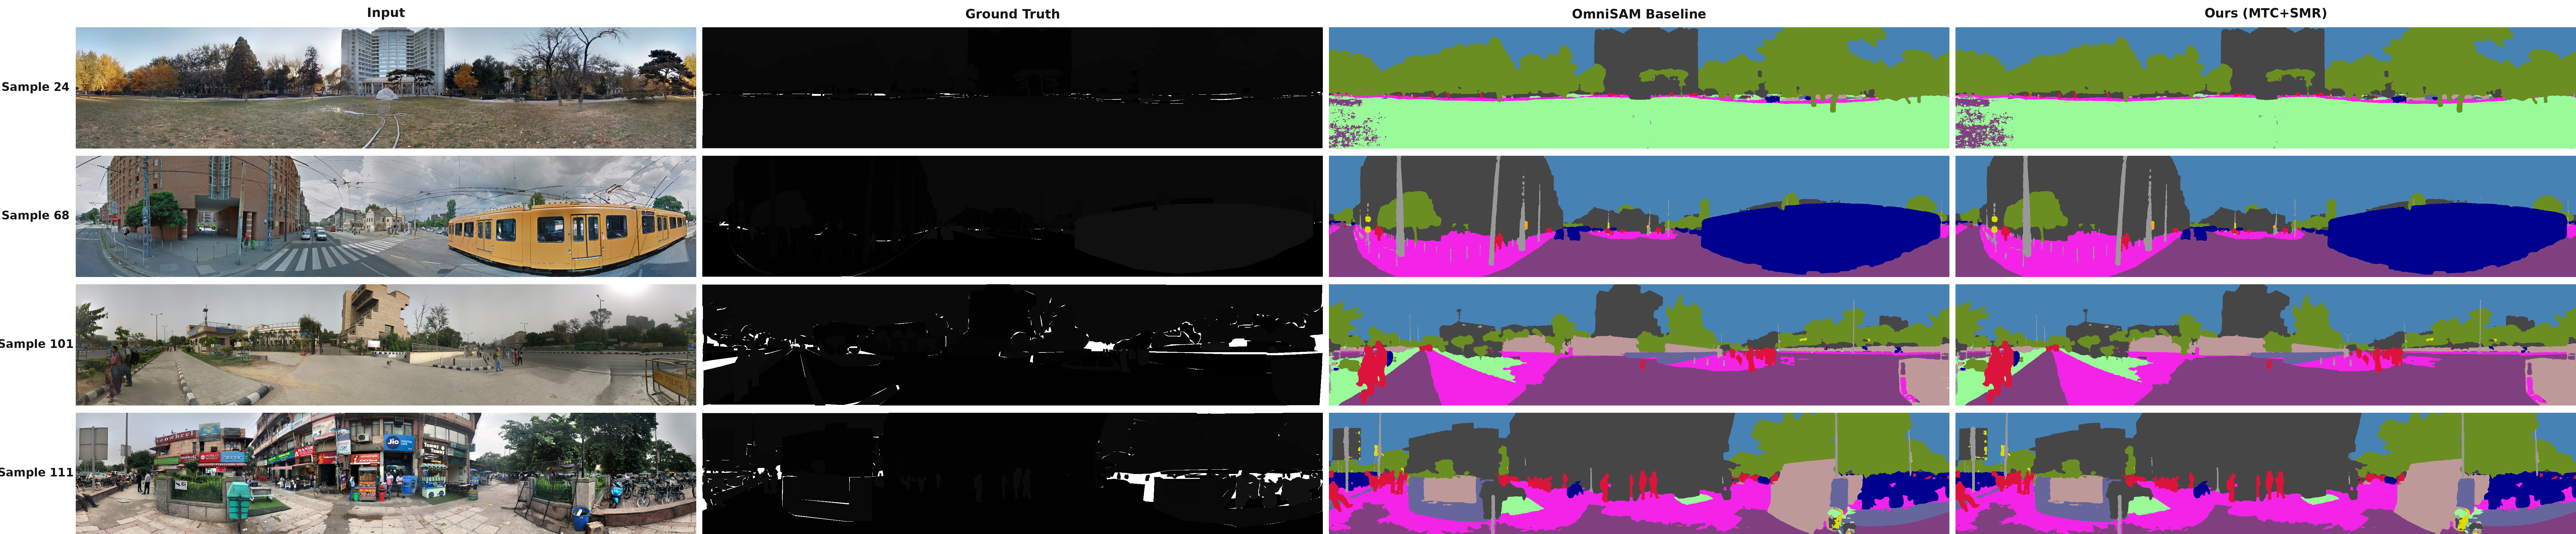
\includegraphics[width=0.95\linewidth]{figures/fig_qualitative_full_protocol.png}
\caption{定性结果对比。从上到下：原始全景图像、OmniSAM（仅Memory优化）、完整方法（Memory+SCM）的分割结果。红框标注处显示边界连续性的改善。}
\label{fig:qualitative_comparison}
\end{figure}

\subsection{效率分析曲线}

图\ref{fig:efficiency_curves}展示了记忆优化的速度-精度权衡曲线。左图显示Token预算与注意力时间的关系：从100\%基线到12.5\%（8×压缩），注意力时间线性下降。右图显示不同压缩率下的mIoU变化：即使在8×压缩下，精度损失仍控制在0.24\%以内。这些曲线验证了我们方法在大范围压缩率下的鲁棒性。

\begin{figure}[t]
\centering
\begin{subfigure}{0.48\linewidth}
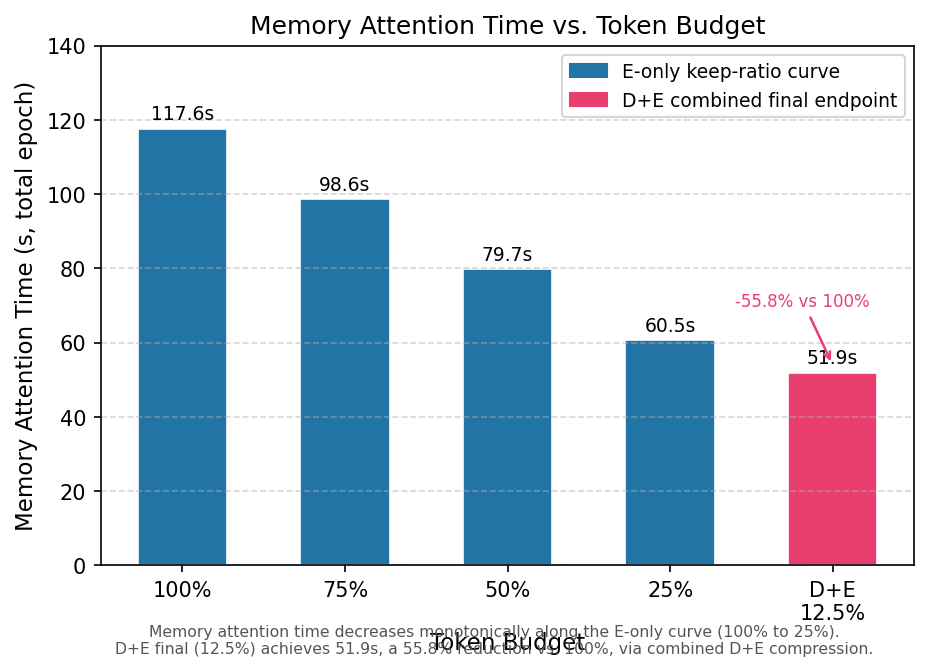
\includegraphics[width=\linewidth]{figures/fig_token_budget_attention_time.png}
\caption{Token预算与注意力时间}
\end{subfigure}
\hfill
\begin{subfigure}{0.48\linewidth}
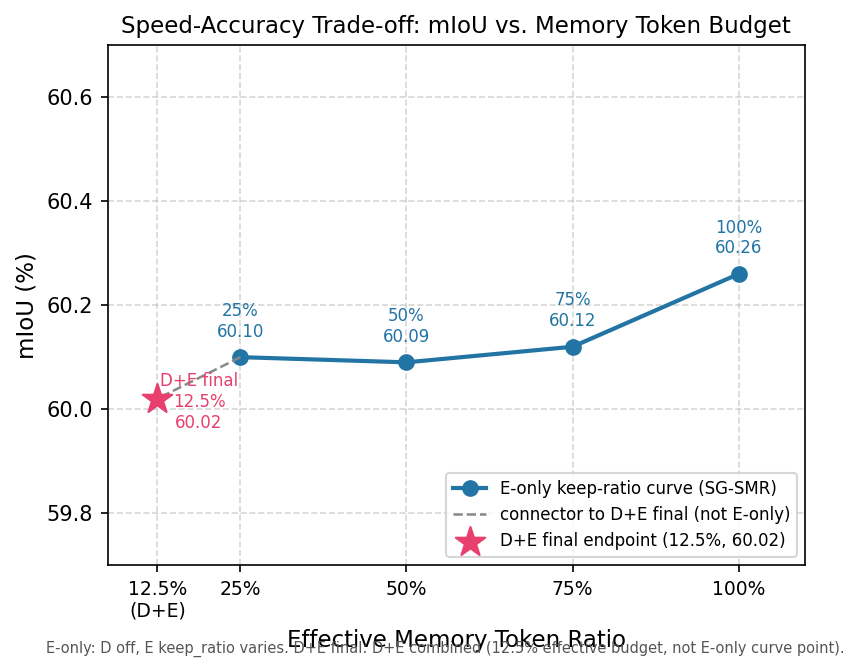
\includegraphics[width=\linewidth]{figures/fig_speed_accuracy_tradeoff_miou.png}
\caption{速度-精度权衡曲线}
\end{subfigure}
\caption{记忆优化的效率分析曲线。(a) 不同Token预算下的注意力计算时间；(b) 压缩率与mIoU的权衡关系。}
\label{fig:efficiency_curves}
\end{figure}
